\documentclass{article}
\usepackage[utf8]{inputenc}
\usepackage{graphicx}
\usepackage{mathtools} 
\usepackage{textcomp}
\usepackage{titling}
\usepackage{subfig}
\usepackage{amsmath}
\usepackage[parfill]{parskip}
\usepackage{xcolor}
\definecolor{LightGray}{gray}{0.9}
\usepackage{titlesec}
\setcounter{secnumdepth}{4}
\usepackage[a4paper,left=1cm,right=1cm,top=1cm,bottom=1.5cm,]{geometry}
\usepackage{eqparbox}
\usepackage{enumitem}

\title{\vspace{-2cm} Dynamic Latches}
\date{\vspace{-5ex}}

\begin{document}
\maketitle
\section{Introduction}
Dynamic latches are based upon \textbf{temporary} storage of charge on parasitic capacitances,
as opposed to static latches which utilize feedback.

Hence, periodic refresh of logic value is necessary to overcome any leakage, and reading of stored value should be \textbf{non-destructive}.

More advanced dynamic latches such as $C^{2}MOS$ or $TSPC$ dynamic latches are not covered.


\section{Dynamic edge-triggered (ET) register}
\begin{minipage}[c]{0.6\textwidth}
    \vspace{0pt}
    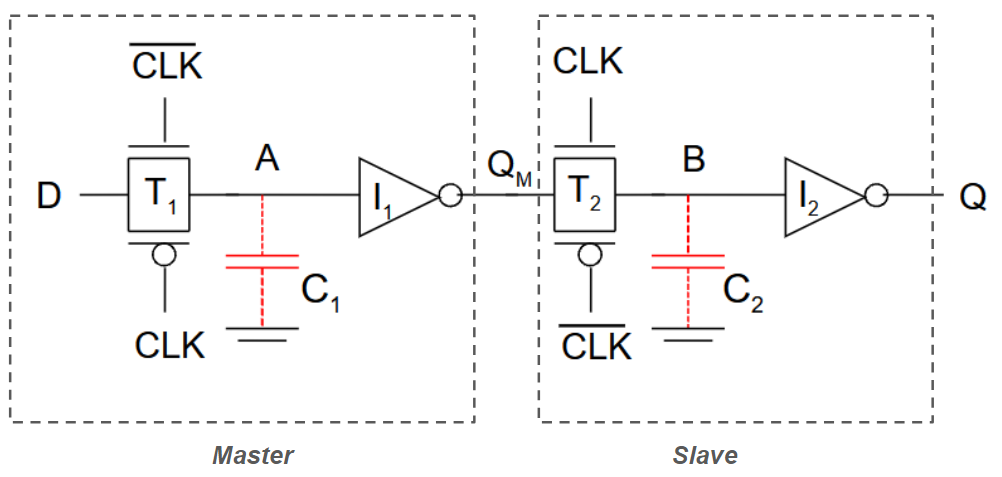
\includegraphics[width=12cm, scale=1]{etRegisterOverview.PNG}
    \captionof{figure}{Dynamic ET register\\
                        (Positive edge-triggered)}
\end{minipage}%
\begin{minipage}[c]{0.5\textwidth}
    \vspace{0pt}
    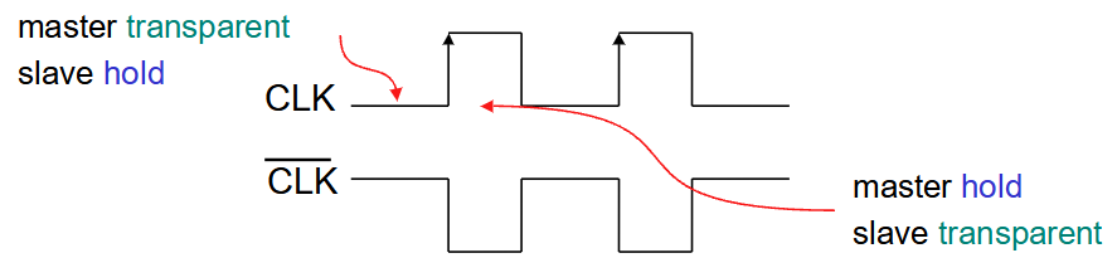
\includegraphics[width=8cm, scale=1]{timingOverview.PNG}
    \captionof{figure}{Master-Slave timing}
\end{minipage}

\begin{itemize}
    \item $t_{setup} = t_{PD,t_{1}} + t_{INV,I_{1}}$
    \item $t_{hold} = 0$
    \item $t_{clk-q} = t_{PD,t_{2}} + t_{INV,I_{2}}$
\end{itemize}

\vspace{1cm}
\subsection{Race problems}
\begin{minipage}[t]{0.5\textwidth}
    \centering
    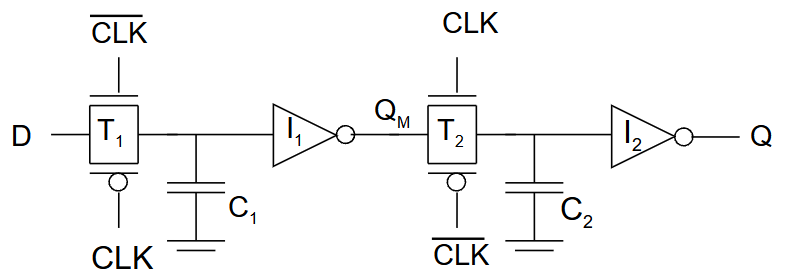
\includegraphics[width=10cm, scale=1]{registerRace.PNG}
    \captionsetup{justification=centering}
    \captionof{figure}{Dynamic ET register}
\end{minipage}%
\begin{minipage}[t]{0.5\textwidth}
    \centering
    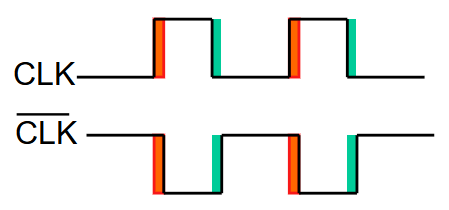
\includegraphics[width=6cm, scale=1]{raceClock.PNG}
    \captionsetup{justification=centering}
    \captionof{figure}{Overlapping clocks\\
                        Green=\textit{0-0}, Red=\textit{1-1}}
\end{minipage}%

\begin{itemize}
    \item \textit{0-0} overlap race
        \begin{itemize}
            \item Suppose $\overline{CLK} = CLK = 0$
            \item $T_{1}$ turns on (more accurately, PMOS side controlled via CLK will be ON)
                \begin{itemize}
                    \item Master latch goes transparent and samples D
                \end{itemize}
            \item However, $T_{2}$ \textbf{wrongfully} turns on (more accurately, PMOS side controlled via $\overline{CLK}$ will be ON). 
                \begin{itemize}
                    \item Slave latch goes transparent and samples $Q_{M}$ (which is actually D)
                \end{itemize}
            \item D therefore wrongly overwrites sampled data on $C_{2}$
            
            \newpage
            \item \textbf{Cannot} be solved by using non-overlapping clocks

                \begin{minipage}[t]{0.4\textwidth}
                    \centering
                    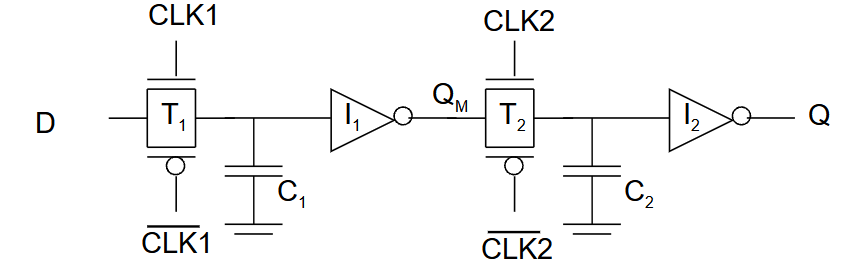
\includegraphics[width=9cm, scale=1]{nonOverlap_fail1.PNG}
                    \captionsetup{justification=centering}
                    \captionof{figure}{Non-overlapping clocks}
                \end{minipage}%
                \begin{minipage}[t]{0.6\textwidth}
                    \centering
                    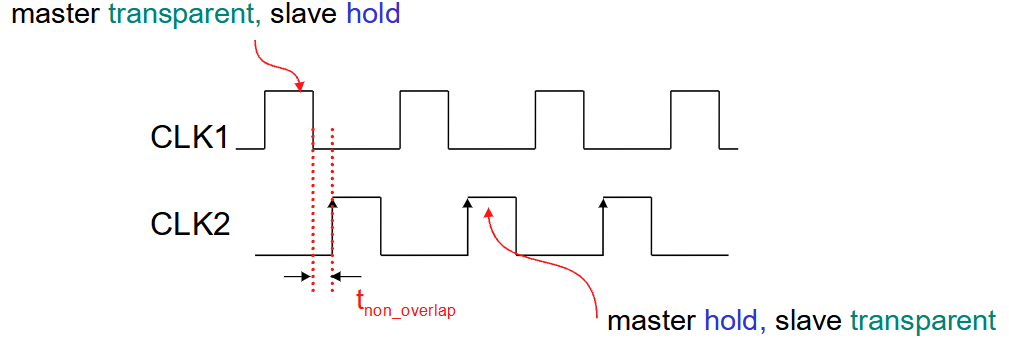
\includegraphics[width=10cm, scale=1]{nonOverlap_fail2.PNG}
                    \captionsetup{justification=centering}
                    \captionof{figure}{\textit{0-0} overlap still exists}
                \end{minipage}%

            \vspace{0.5cm}
            \item Can be solved by increasing $t_{setup}$

            \begin{minipage}[c]{0.4\textwidth}
                \centering
                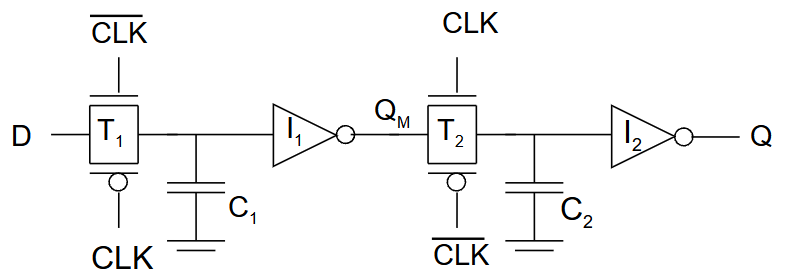
\includegraphics[width=8cm, scale=1]{registerRace.PNG}
                \captionsetup{justification=centering}
                \captionof{figure}{Dynamic ET register}
            \end{minipage}%
            \begin{minipage}[c]{0.6\textwidth}
                \centering
                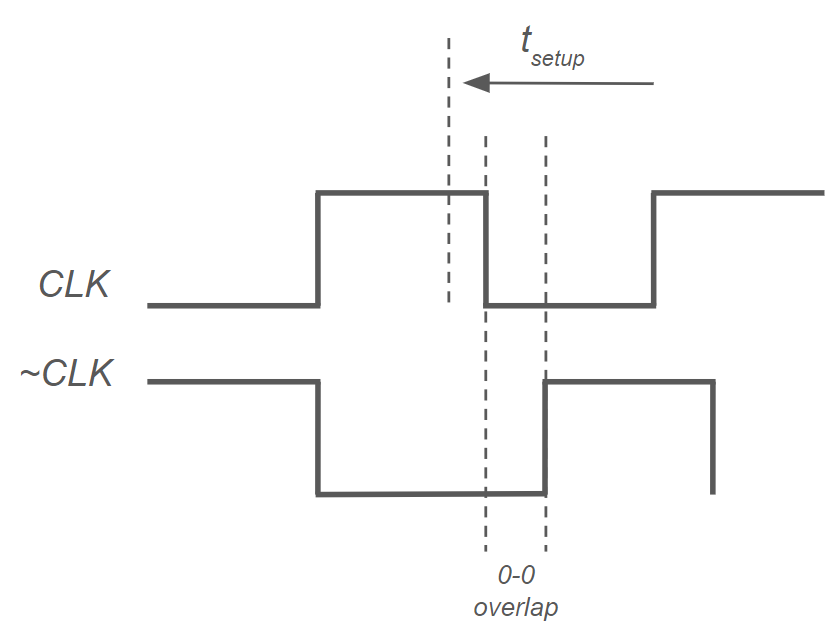
\includegraphics[width=7cm, scale=1]{setupfix.PNG}
                \captionsetup{justification=centering}
                \captionof{figure}{Setup time}
            \end{minipage}%

            \begin{itemize}
                \item $T_{1}$ is a \textbf{negative} latch, but ET register is \textbf{positive} edge-triggered
                \item $t_{setup}$ can be increased by increasing $t_{PD,t_{1}}$
                \item Intuitively, we do not allow D to change within the \textit{0-0} overlap period, which solves the issue
                \item Alternatively, we can understand that via increasing $t_{PD,t_{1}}$, $D_{sampled}$ from transparent $T_{1}$ takes a longer time to travel to $T_{2}$.
                        If it takes sufficiently long enough, by the time $D_{sampled}$ reaches $T_{2}$, we will already be outside of the \textit{0-0} overlap zone, and $T_{2}$ is in hold mode.
            \end{itemize}
        \end{itemize}
    \item \textit{1-1} overlap race
        \begin{itemize}
            \item Suppose $\overline{CLK} = CLK = 1$
            \item $T_{1}$ \textbf{wrongfully} turns on (more accurately, NMOS side controlled via $\overline{CLK}$ will be ON)
                \begin{itemize}
                    \item Master latch goes transparent and samples D
                    \item But, $T_{2}$ is currently transparent and sampling from $Q_{m}$
                    \item $D_{sampled}$ may overwrite data on $C_{1}$, and corrupt what $T_{2}$ is sampling
                \end{itemize}

            \vspace{0.5cm}
            \item Can be solved by increasing $t_{hold}$
            
            \begin{minipage}[c]{0.4\textwidth}
                \centering
                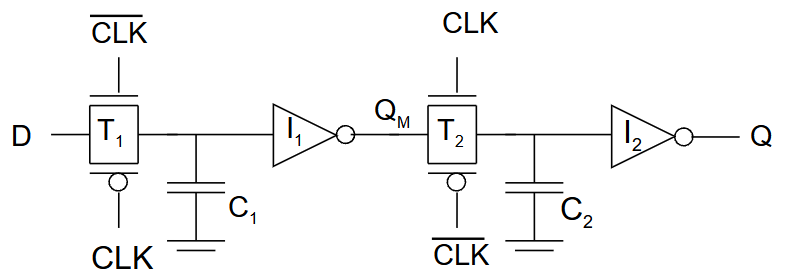
\includegraphics[width=8cm, scale=1]{registerRace.PNG}
                \captionsetup{justification=centering}
                \captionof{figure}{Dynamic ET register}
            \end{minipage}%
            \begin{minipage}[c]{0.6\textwidth}
                \centering
                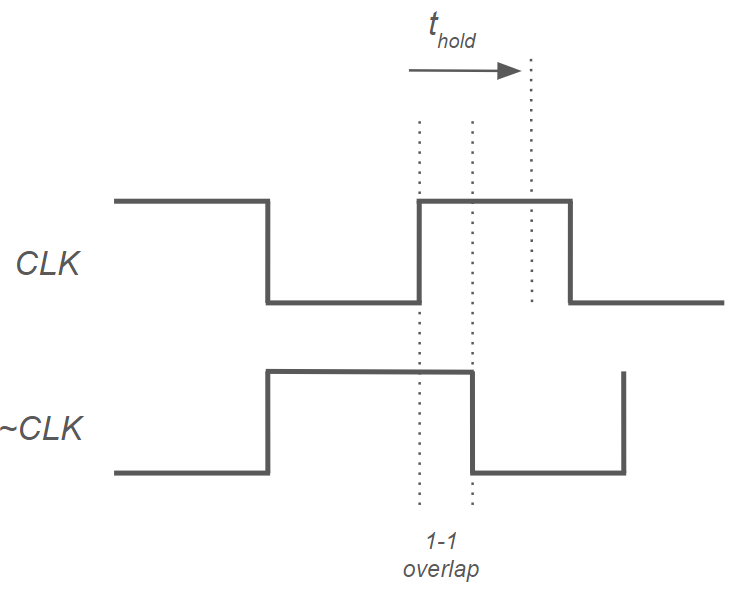
\includegraphics[width=6cm, scale=1]{holdtime.PNG}
                \captionsetup{justification=centering}
                \captionof{figure}{Hold time}
            \end{minipage}%
                \begin{itemize}
                    \item D is only allowed to change \textbf{after} $\overline{CLK}$ becomes 0
                \end{itemize}
        \end{itemize}
\end{itemize}



\end{document}